\chapter{Datos: EDA y preprocesamiento}

En este capítulo discutiremos los distintos detalles de la implementación de nuestro sistema: desde el preprocesamiento de los datos hasta la elección y entrenamiento del modelo.


\section{Datos: fuente y forma}
Los datos escogidos provienen del dataset \href{https://www.kaggle.com/chaitanyakck/medical-text}{Medical Text} publicado por Chaitanya Krishna Kasaraneni, y de \href{https://www.kaggle.com/tboyle10/medicaltranscriptions}{Medical Transcriptions}, publicado por Tara Boyle. La naturaleza de los mismos es ligeramente diferente así que explicaremos el proceso de preprocesamiento y unificación posteriormente.

\subsection{Medical Text}
El dataset tiene formato \jesitt{.dat}, estructurado como un \jesitt{.tsv} (Tab Separated Values). La primera columna corresponde con una categoría determinada --ya que el dataset estaba diseñado para clasificación-- y la segunda columna contiene fragmentos de documentos médicos.

El dataset está descompuesto en un archivo \jesitt{train.dat} y otro \jesitt{test.dat}. El archivo de entrenamiento contiene 14438 comentarios, y el de evaluación, 14442. En total, disponemos de 28880 comentarios.

\subsubsection{Análisis de datos exploratorio}
En esta subsección, analizaremos en más profundidad la forma de los datos, para saber qué esperar de cara al entrenamiento de nuestros modelos.

Como podemos observar en las figuras \ref{fig:avg_char_train} y \ref{fig:avg_tokens_train}, la distribución de los distintos elementos de nuestro dataset de entrenamiento está muy normalmente distribuída.

El número medio de caracteres por comentario es de 1230, y el número medio de tokens por comentario es de unos 180, correspondiéndose con las líneas amarillas en las figuras.

Se pueden apreciar, aún así, algunos valores atípicos de comentarios particularmente largos. Esto, sin embargo, no es necesariamente malo en nuestro caso. En definitiva, cuanto más texto tengamos a nuestra disposición, mejor para el modelo.

\begin{figure}[h!]
	\centering
	\begin{subfigure}[t]{0.95\textwidth}
		\centering
		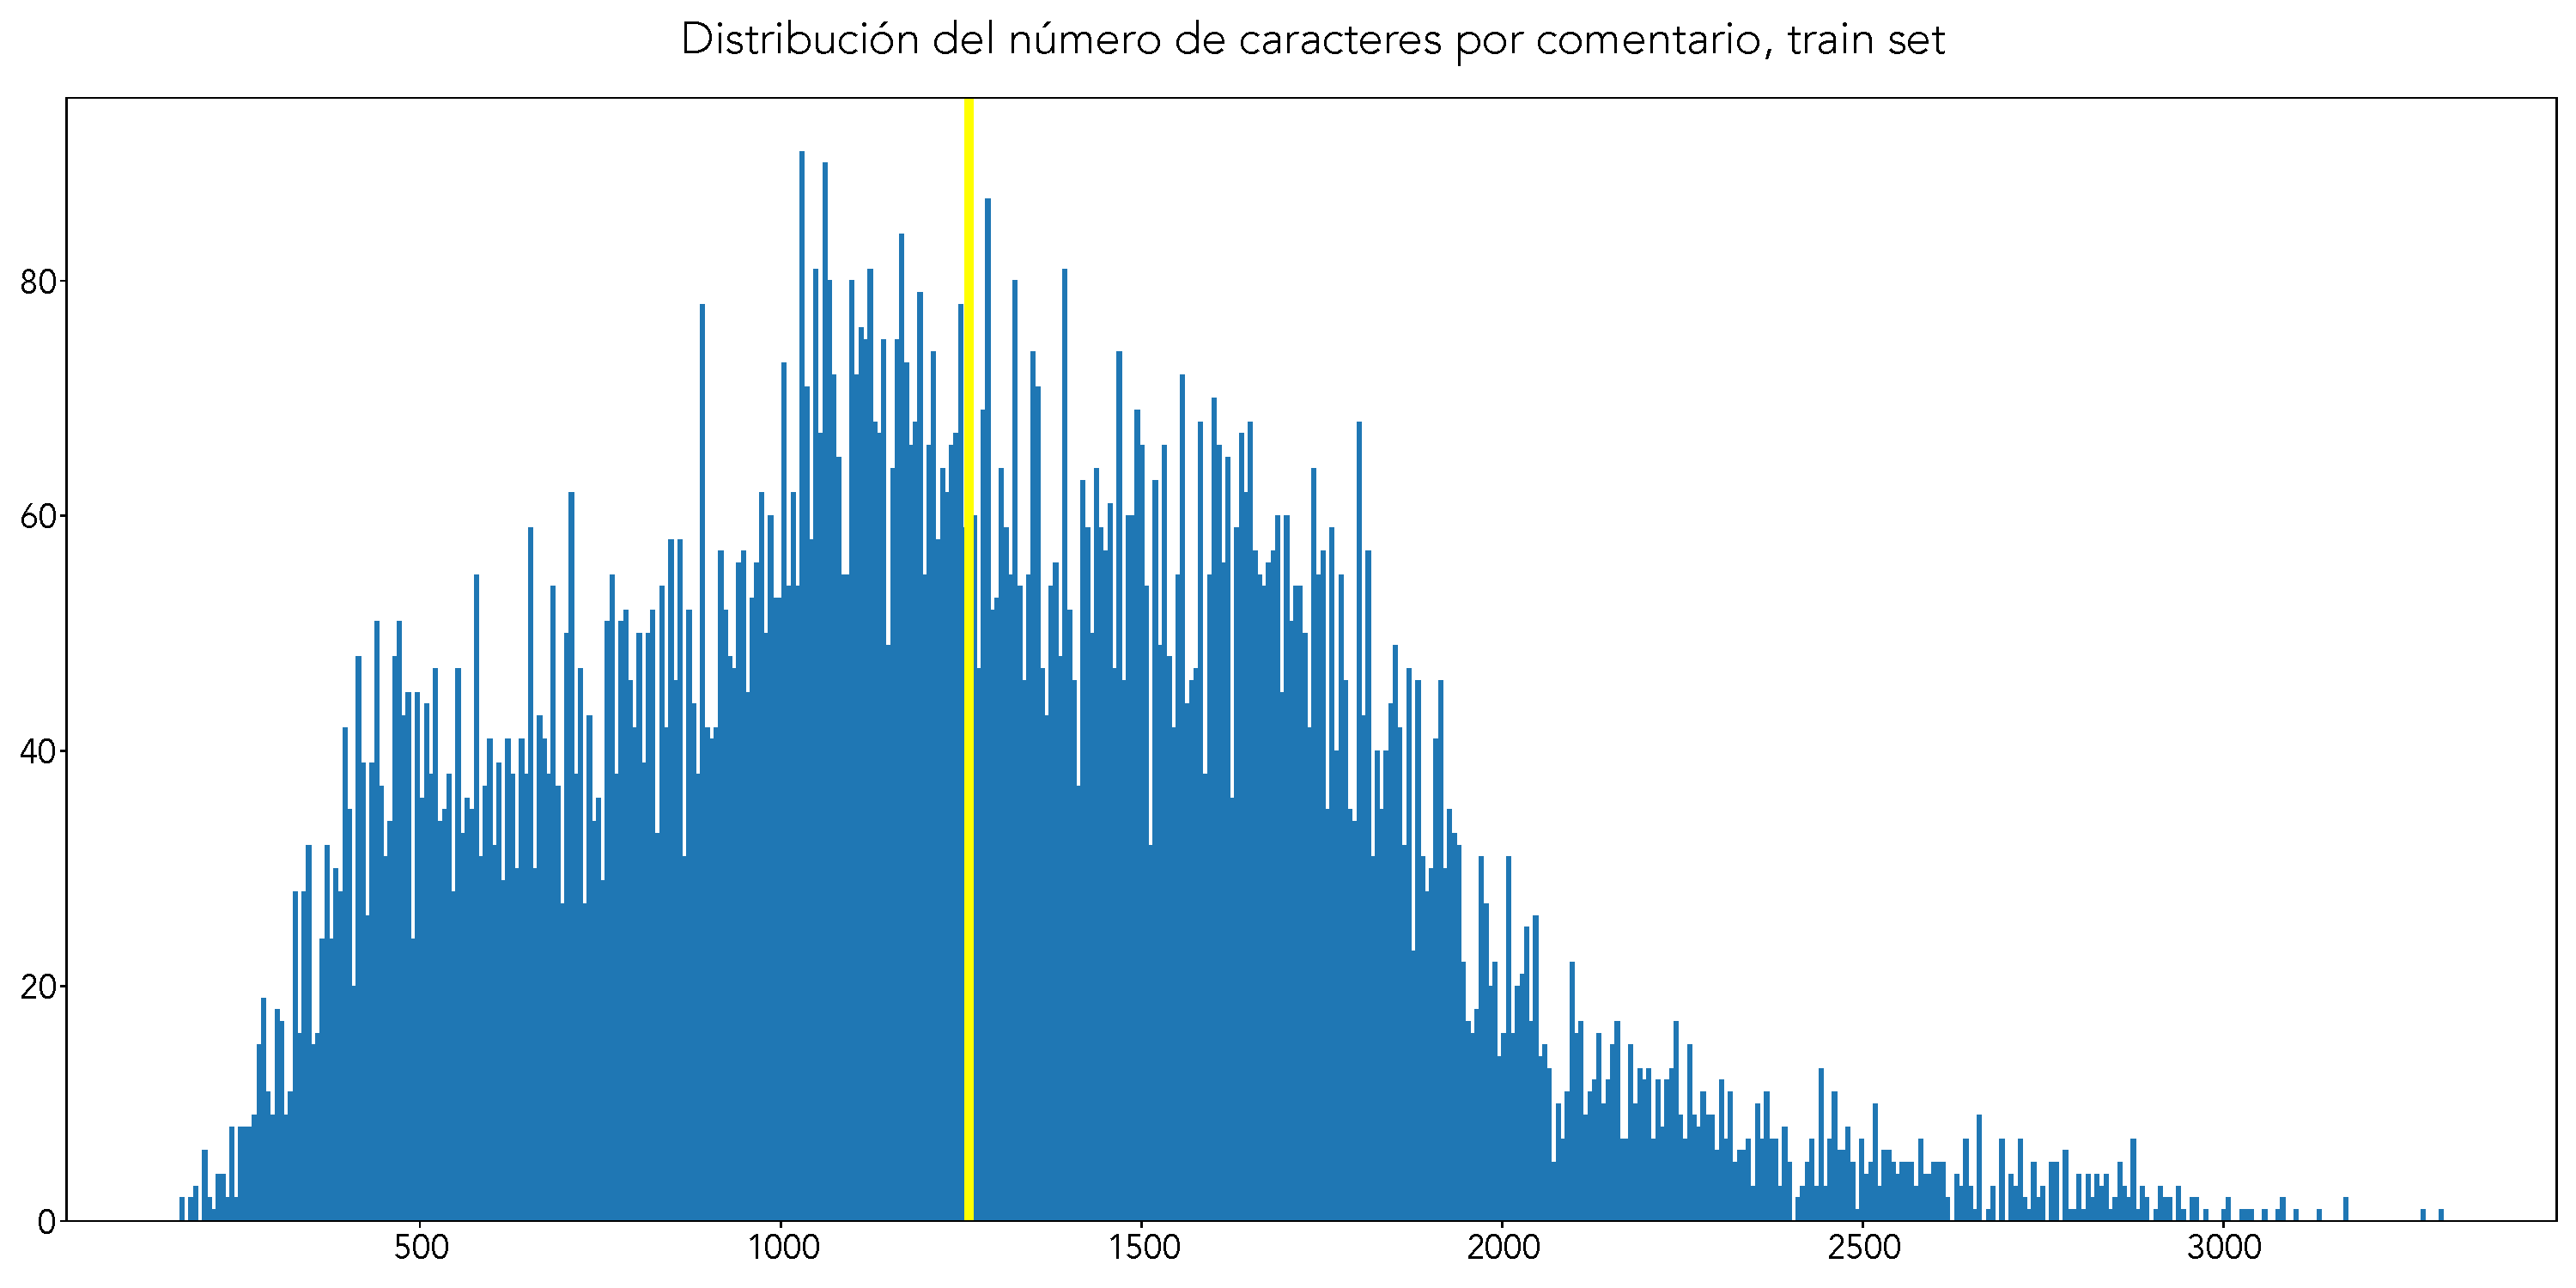
\includegraphics[width=.9\textwidth]{media/char_hist_train.pdf}
		\caption{Distribución del número de caracteres por comentario, en el conjunto de entrenamiento}
		\label{fig:avg_char_train}
	\end{subfigure}
	~

	\begin{subfigure}[t]{0.95\textwidth}
		\centering
		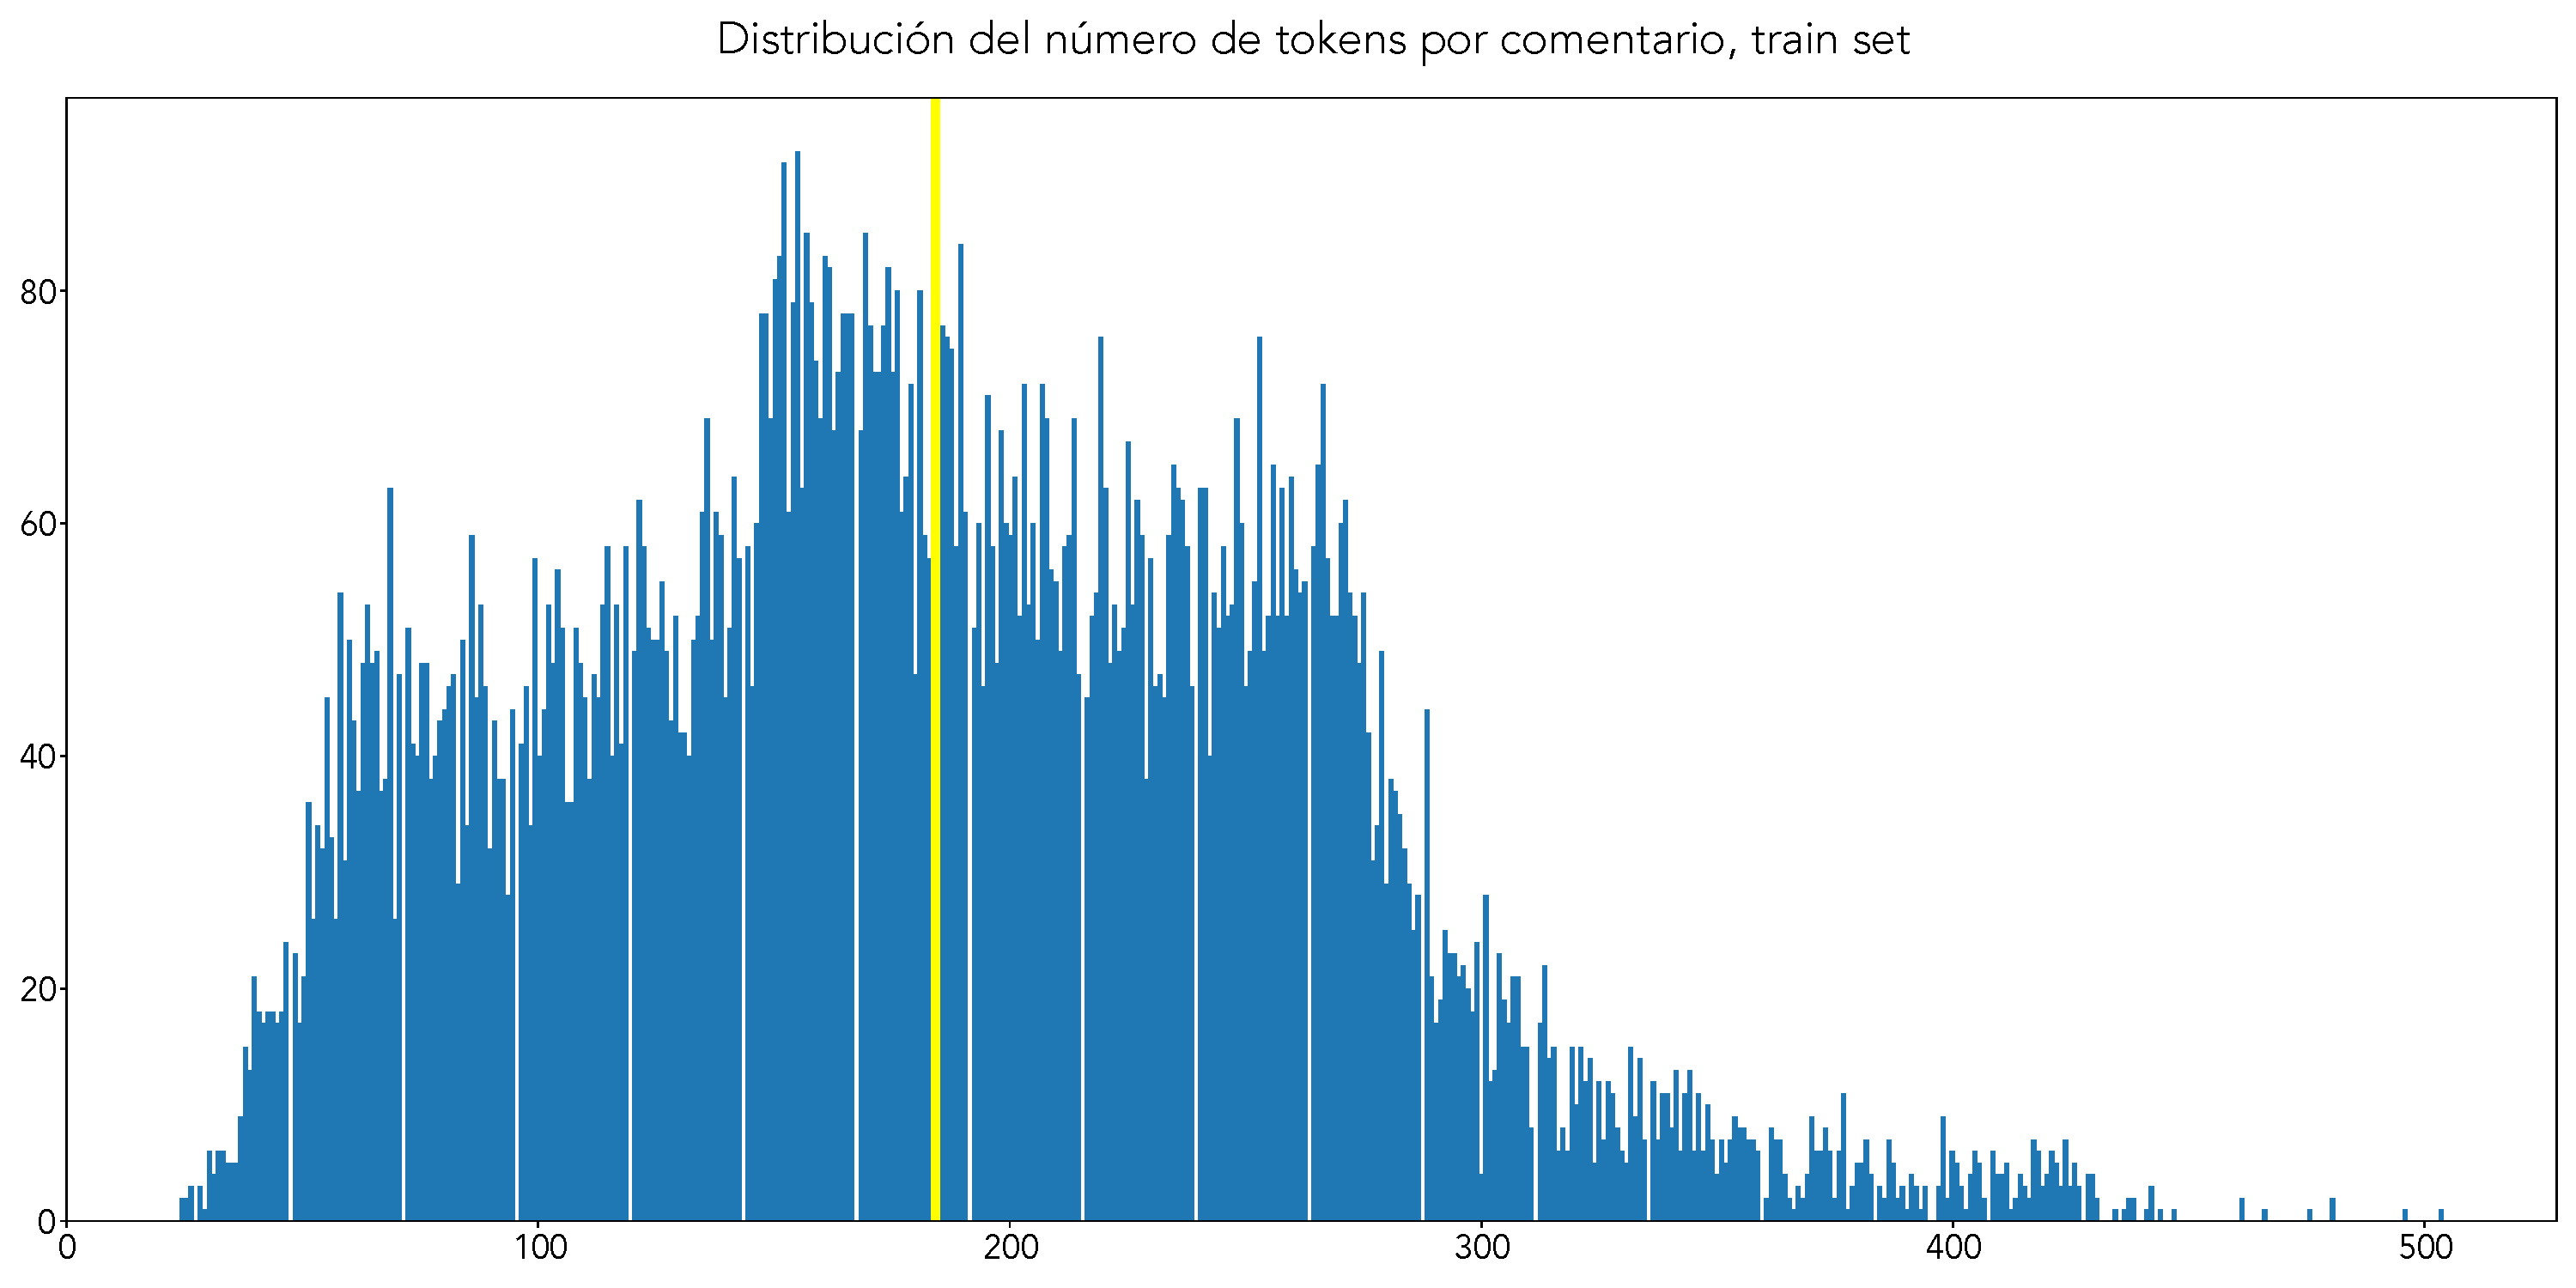
\includegraphics[width=.9\textwidth]{media/tokens_hist_train.pdf}
		\caption{Distribución del número de tokens por comentario en el conjunto de entrenamiento}
		\label{fig:avg_tokens_train}
	\end{subfigure}

	\caption{Visualización de la distribución de nuestro conjunto de entrenamiento}
	\label{fig:sum_train}
\end{figure}


\begin{figure}[h!]
	\centering
	\begin{subfigure}[t]{0.95\textwidth}
		\centering
		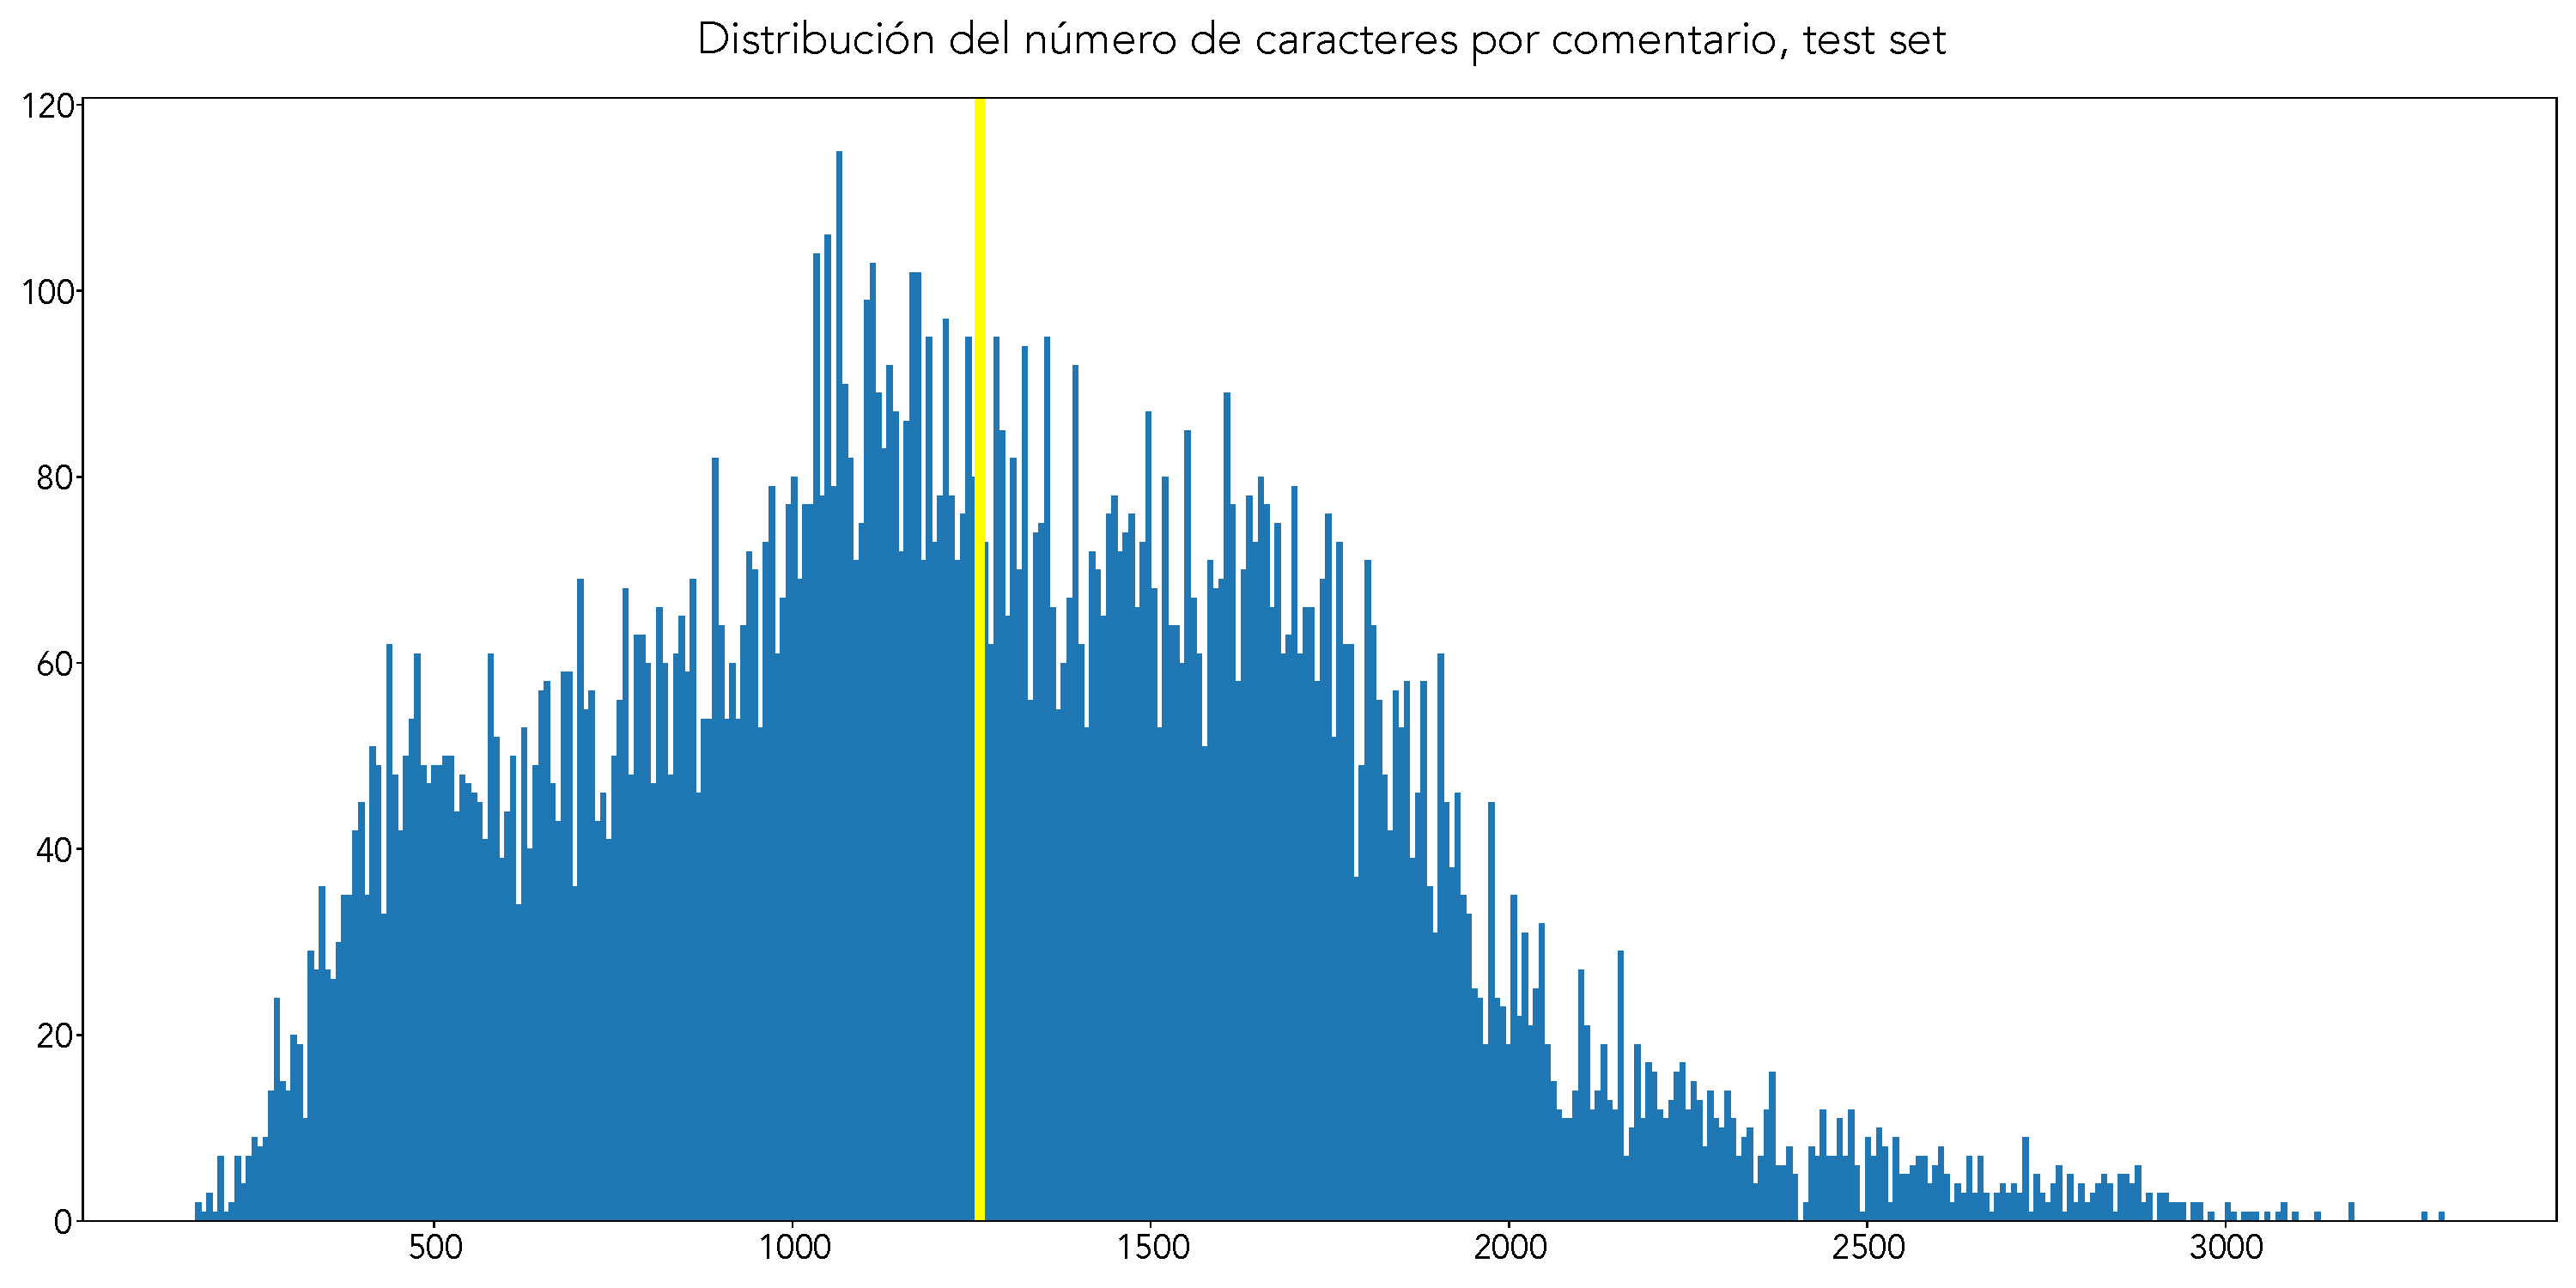
\includegraphics[width=.9\textwidth]{media/char_hist_test.pdf}
		\caption{Distribución del número de caracteres por comentario, en el conjunto de evaluación}
		\label{fig:avg_char_test_test}
	\end{subfigure}

	~

	\begin{subfigure}[t]{0.95\textwidth}
		\centering
		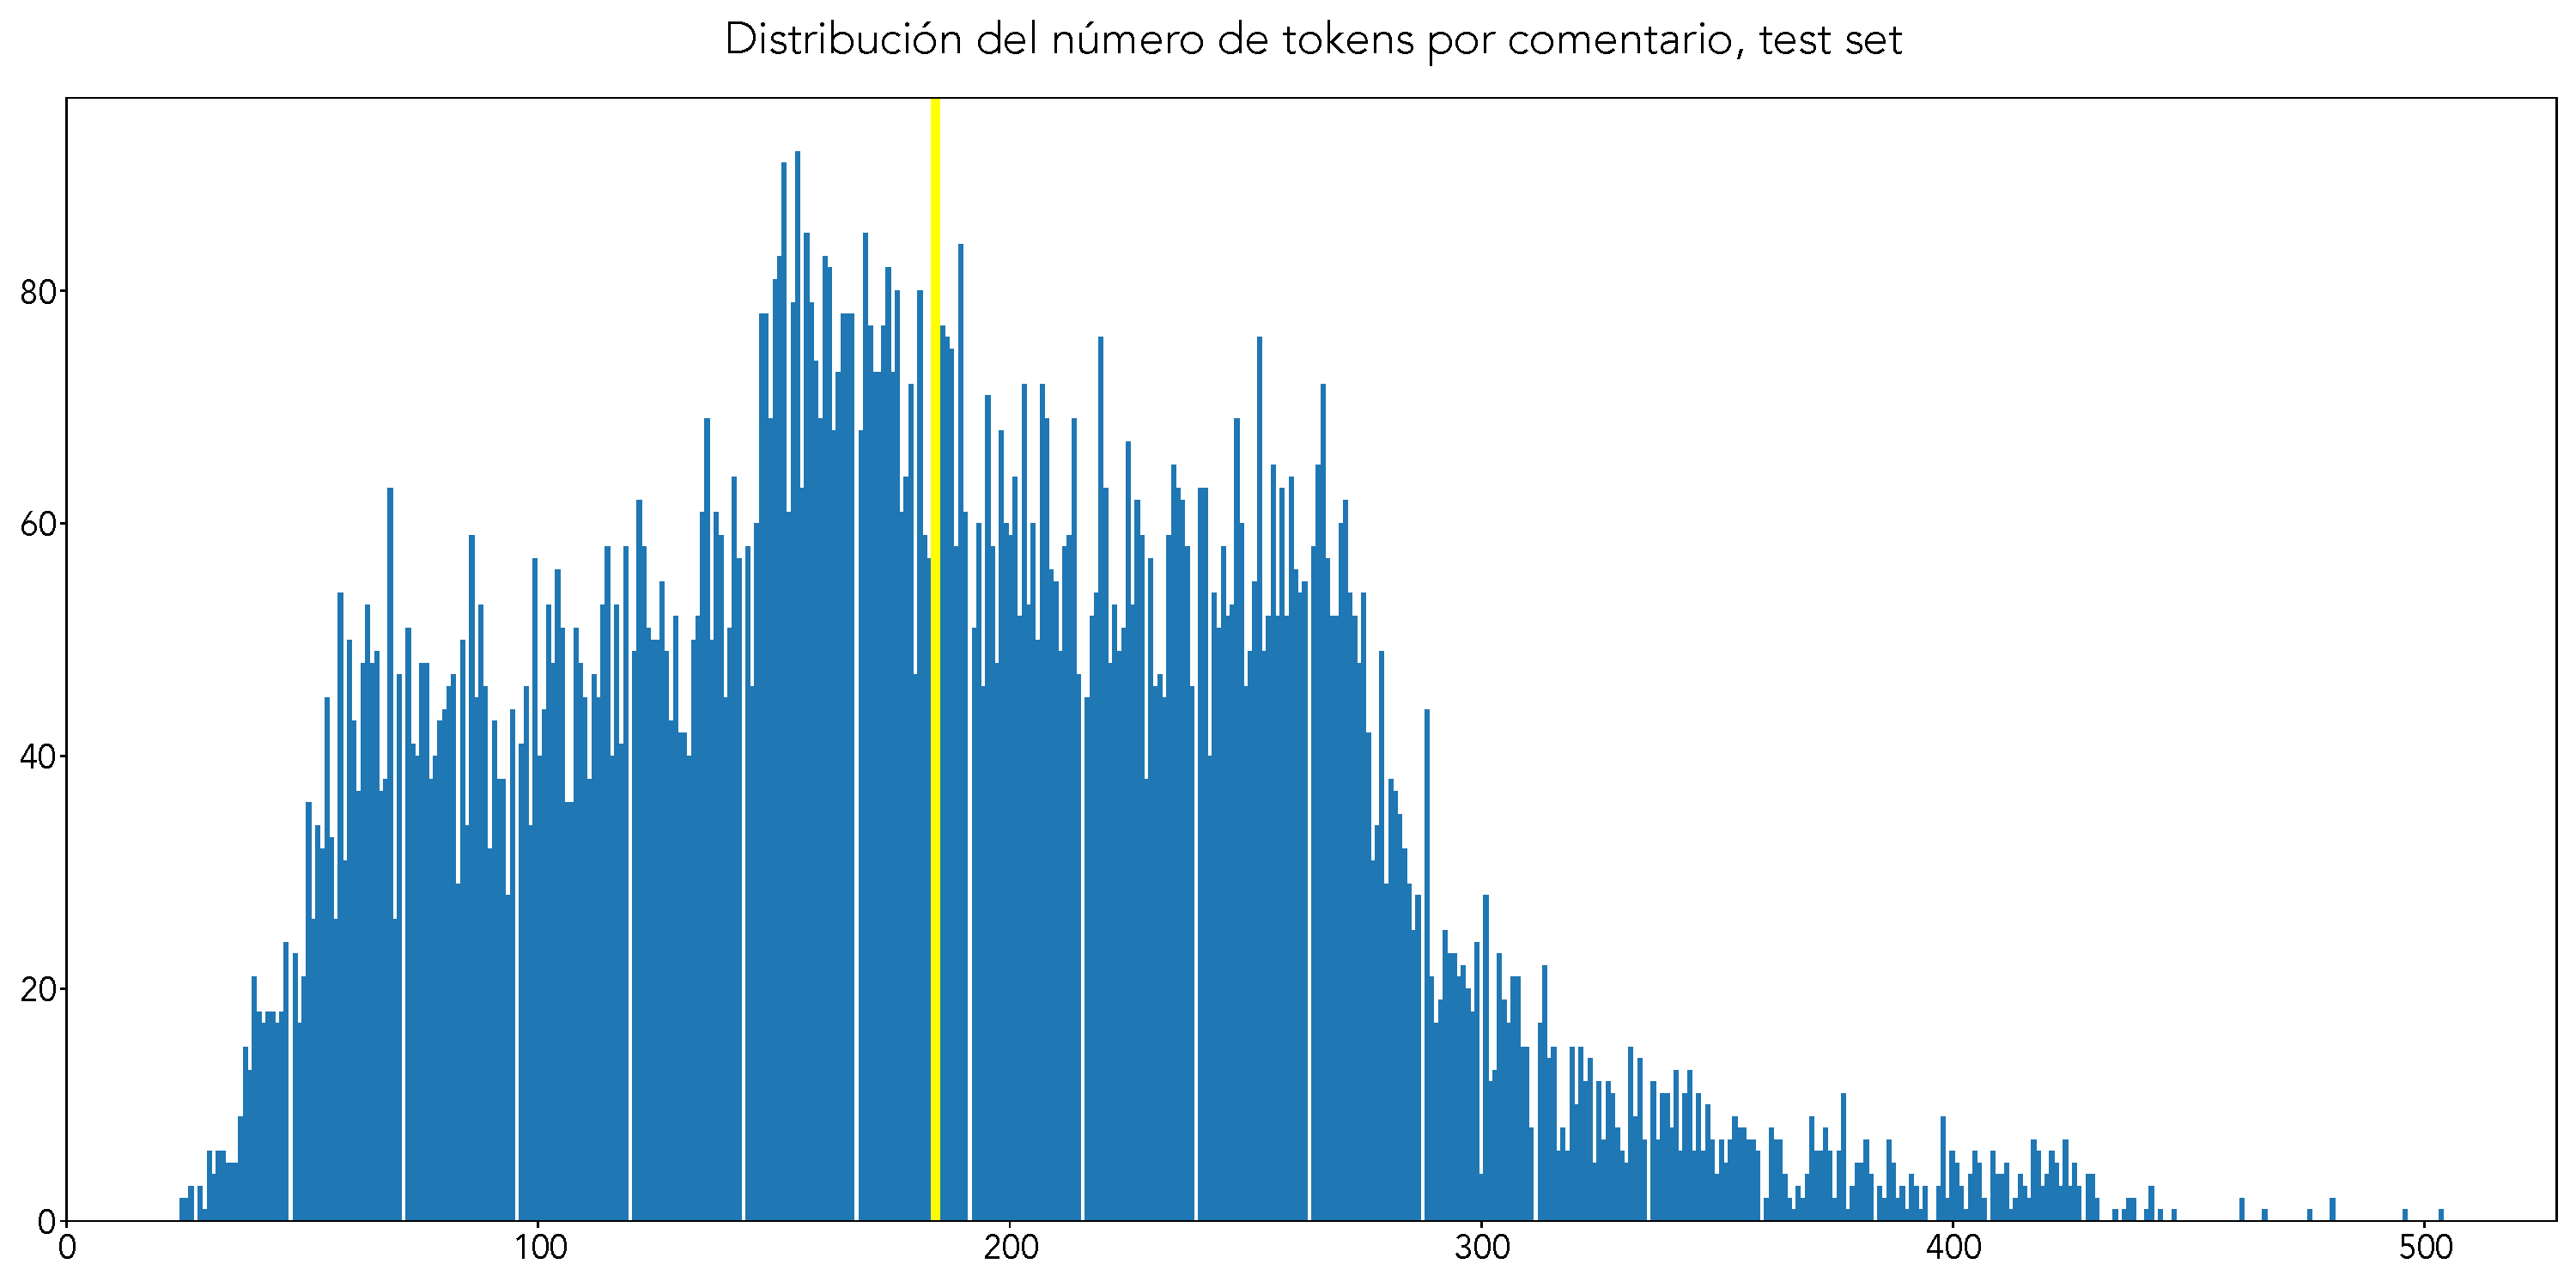
\includegraphics[width=.9\textwidth]{media/tokens_hist_test.pdf}
		\caption{Distribución del número de tokens por comentario en el conjunto de evaluación}
		\label{fig:avg_tokens_test}
	\end{subfigure}


	\caption{Visualización de la distribución de nuestro conjunto de evaluación}
	\label{fig:sum_test}
\end{figure}

Una media de casi 200 palabras por comentario con comentarios alcanzando las 500 corresponde con comentarios relativamente largos. Esto nos vendrá bien de cara al entrenamiento de nuestro modelo, para poder formar oraciones con más sentido.


\subsection{Medical Transcriptions}
Este dataset es en realidad una extracción de la página web \url{mtsamples.com}, donde se halla una respetable cantidad de trasncripciones médicas. La autora extrajo todos los comentarios, así como los diferentes metadatos que los acompañaban mediante \textit{web scraping} y los provee en la columna \jesitt{trasncription}. 

En este caso, como podemos apreciar en la figura \ref{fig:sum_mdtr}, las distribuciones son ligeramente asimétricas, predominando comentarios más cortos. Aún así, disponemos de comentarios excepcionalmente largos, con alrededor de 18000 caracteres.

\begin{figure}[h!]
	\centering
	\begin{subfigure}[t]{0.95\textwidth}
		\centering
		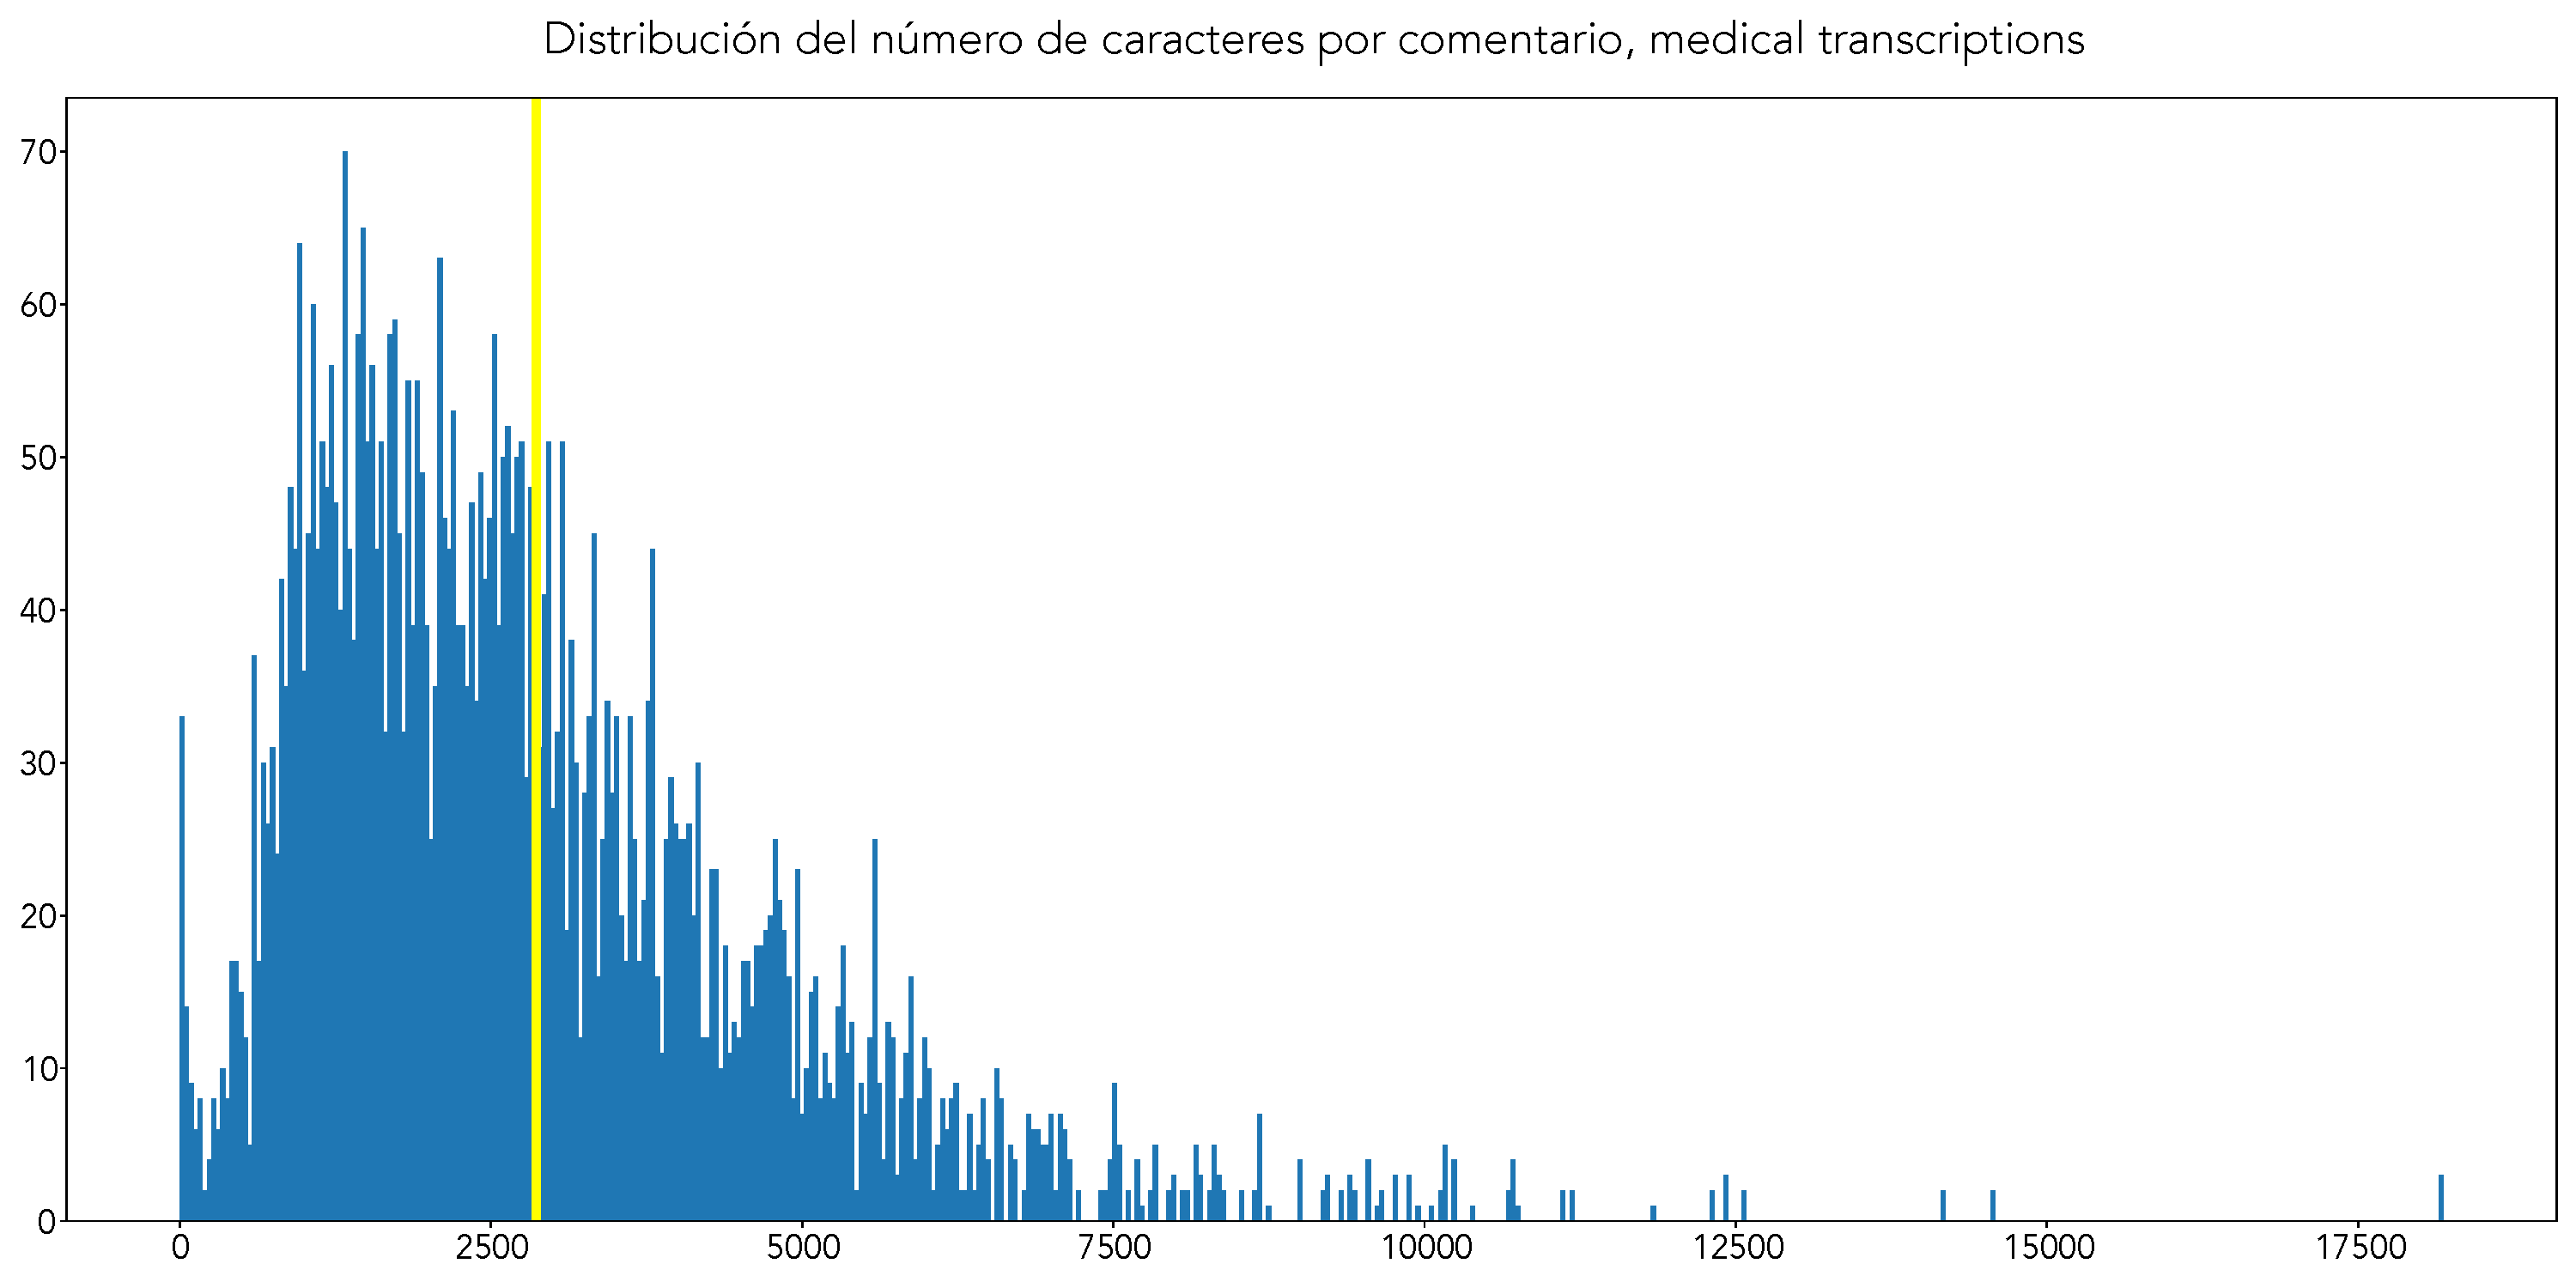
\includegraphics[width=.9\textwidth]{media/char_hist_mdtr.pdf}
		\caption{Distribución de caracteres en el dataset Medical Transcriptions}
		\label{fig:char_hist_mdtr}
	\end{subfigure}

	~
	\begin{subfigure}[t]{0.95\textwidth}
		\centering
		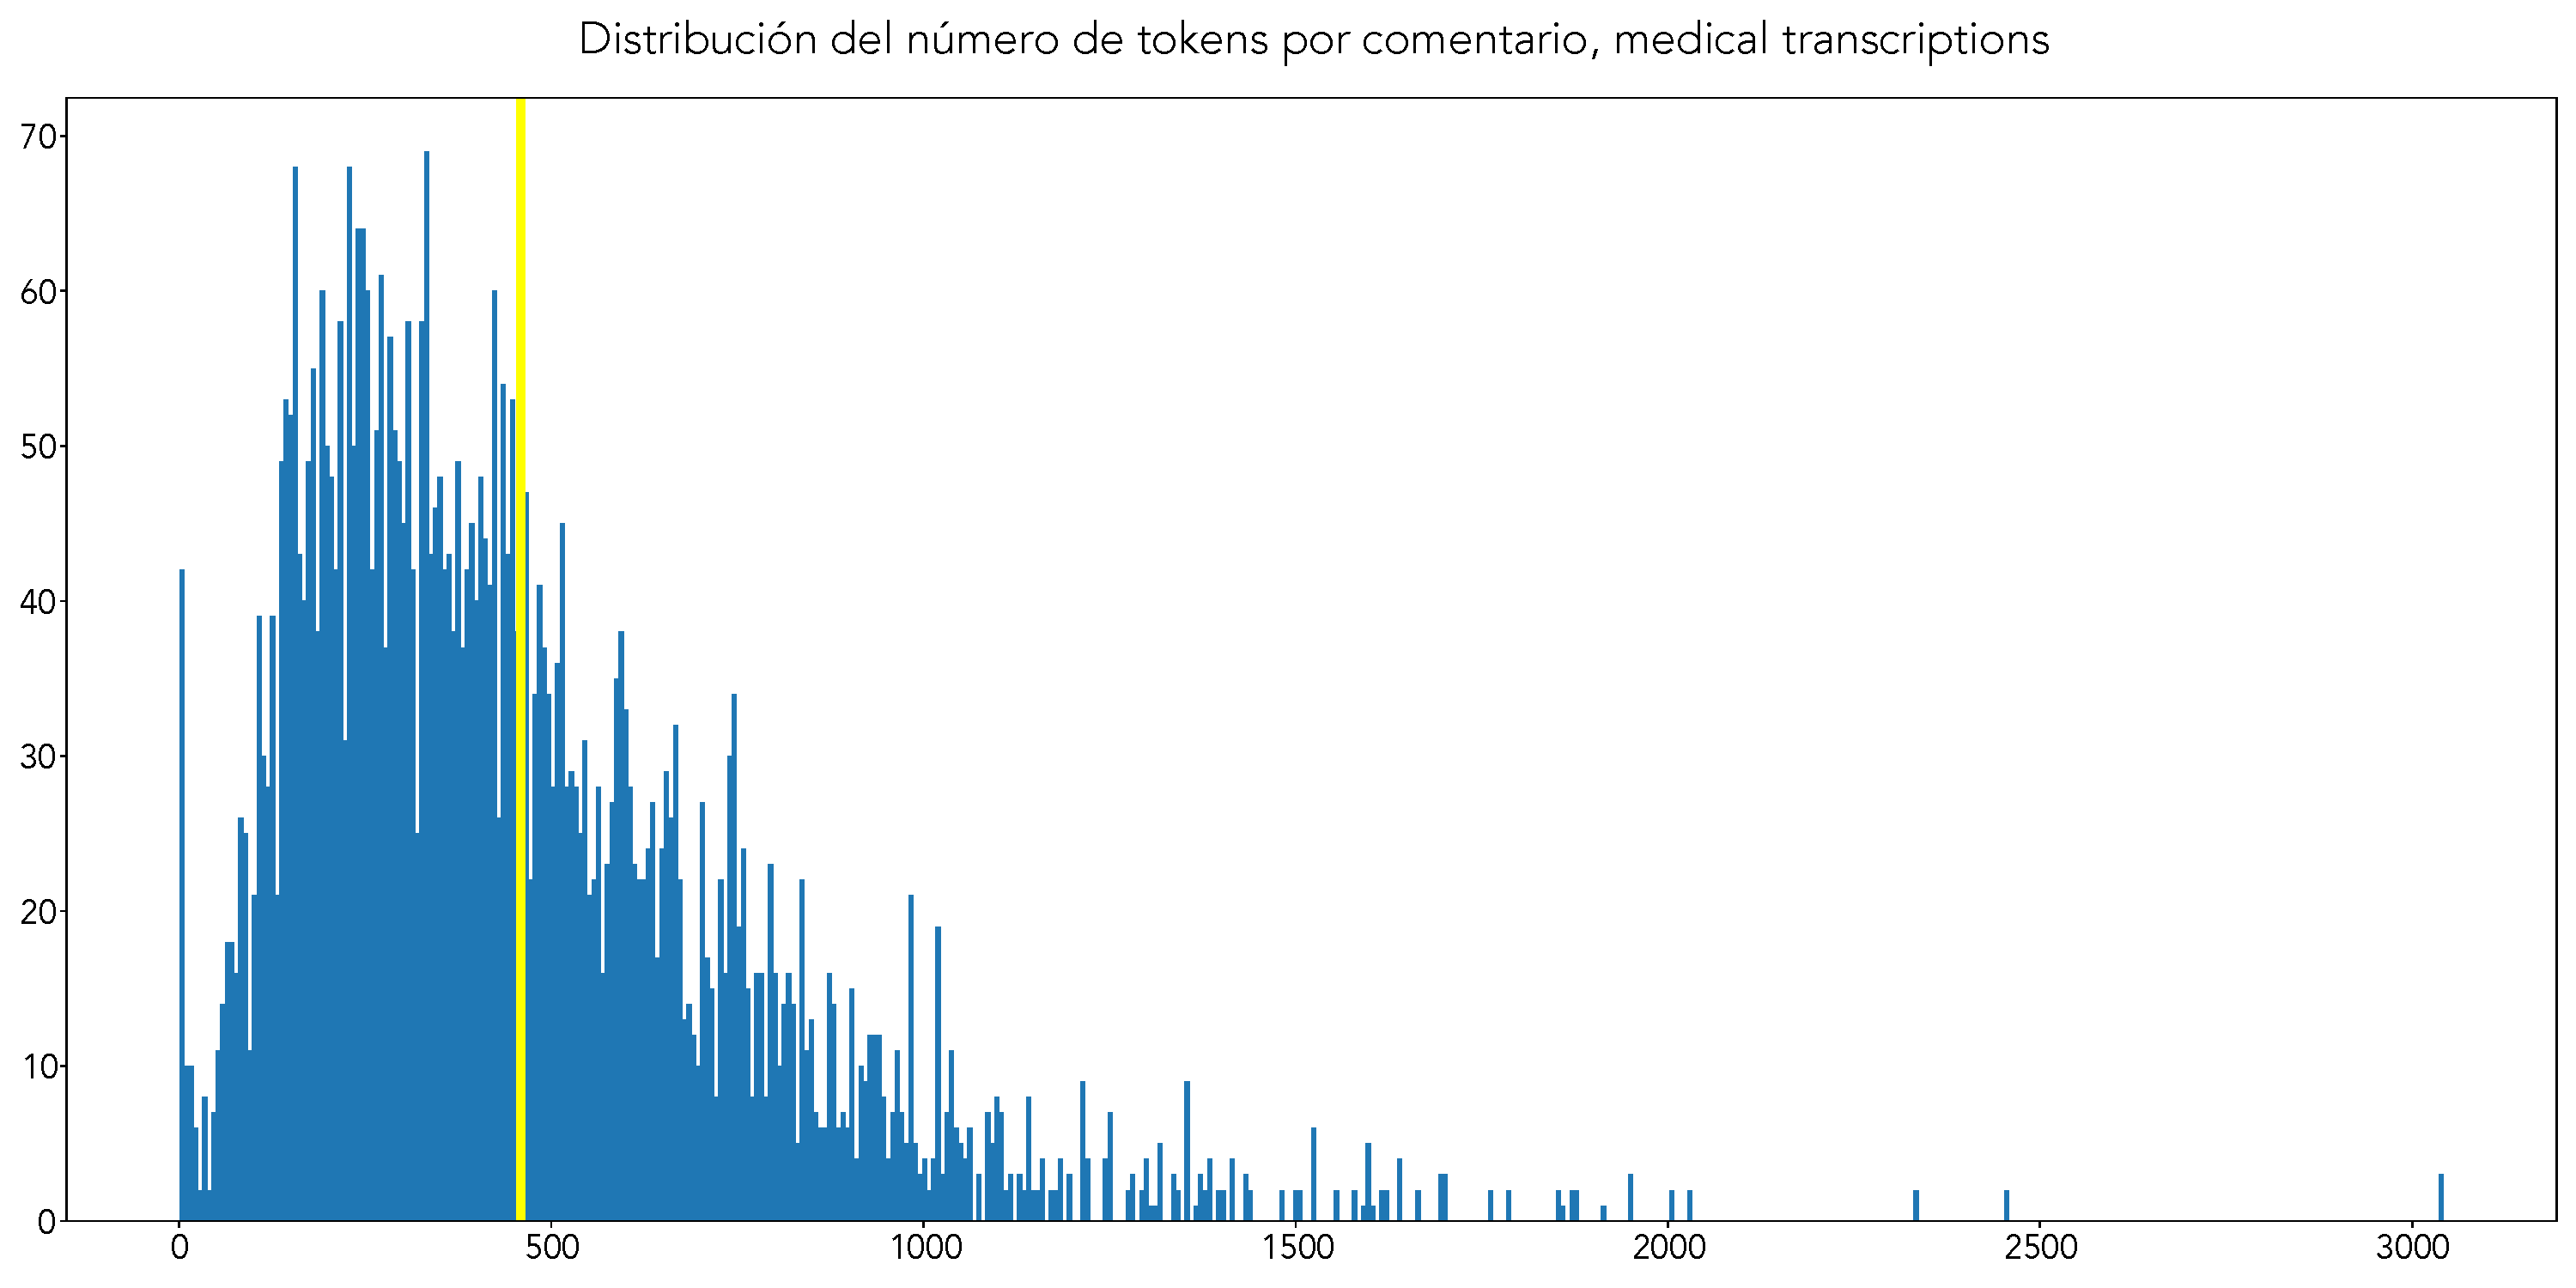
\includegraphics[width=.9\textwidth]{media/token_hist_mdtr.pdf}
		\caption{Distribución de palabras en el dataset Medical Transcriptions}
		\label{fig:token_hist_mdtr}
	\end{subfigure}

	\caption{Visualización del dataset Medical Transcriptions}
	\label{fig:sum_mdtr}
\end{figure}

\section{Preprocesamiento}
En esta sección, describiremos el preprocesamiento acometido en cada uno de los datsets. Provienen de fuentes diferentes así que cada uno recibirá un trato diferente, con objeto de normalizar y unificar el formato de todos de cara al entrenamiento.


\subsection{Medical Text}
Este conjunto de datos, siendo específicamente texto, el formato, ortografía y en general formato de los archivos es muy bueno. Simplemente hemos de eliminar las categorías adjuntas a cada comentario, para obtener una lista de comentarios crudos en sí. Por lo demás, los comentarios carecen de problemas de formato, codificación o cualquier otra cosa que pudiera molestar. Probablemente el autor ya hiciera esto por nosotros antes de publicarlo.


\subsection{Medical Transcriptions}
En el caso de las trancripciones médicas, la tarea es considerablemente más compleja. El conjunto de datos proviene de la página web \url{mtsamples.com}, como especificamos anteriomente. La autora efectuó un proceso de \textit{scraping} para obtener toda la información y recogerla en el archivo \jesitt{.csv}. 

Esto facilita las cosas, pero desde luego los comentarios deben ser profundamente esculpidos antes de pasarlos a cualquier modelo. Los trazos de formato HTML se dejan entrever en los comentarios con signos de puntuación o tabulaciones fuera de lugar, así que debemos arreglarlo previo entrenamiento.

Para ello, se ha hecho un fuerte uso de expresiones regulares, y se ha creado un pequeño \textit{pipeline} para procesar todo el texto a la vez.

El pipeline elimina todas las posibles trazas o residuos que hubieran quedado del \textit{scraping}. Este es el pipeline:

\begin{minted}[breaklines, linenos]{python}
def regex_processing(text):
    # Remove capital letters surrounded by 0 or more `,` and a colon, i.e. the titles
    no_caps = re.sub(r',*([A-Z\s]+):', '', text)

    # Remove weirdly positioned commas. Find commas that dont have any letter before and some space after them.
    weird_commas = re.sub(r'(?<!\w),\s+', '', no_caps)
    
    # Remove commas that dont have spaces around them. (Commas should always have a trailing space after them)
    more_commas = re.sub(r'(?<!\s),(?!\s)', ' ', weird_commas)

    # Remove digits adyacent to dots or commas, as in enumerated lists.
    no_digits = re.sub(r'[\.,]*\d[\.,]+', ' ', more_commas)

    # Remove any other commas left behind the process. Particularly these cases: Hello. ,How are you?
    trailing_commas = re.sub(r'\s,(?=[A-Z\d])', '', no_digits)

    # Substitute any number of spaces for 1 single space.
    no_double_spaces = re.sub(r'\s+', ' ', trailing_commas)

    # Solve these problems: Hello .How are you? => Hello. How are you?
    final_text = re.sub(r'(?<!\s)\.(?!\s)', '. ', no_double_spaces)

    # Finally, strip the text from any trailing commas or white spaces.
    # The result is hopefully a clean version of the text, ready to be tokenized
    # and passed to the models.
    return final_text.strip(', ')
\end{minted}

El resumen del proceso es eliminar signos de puntuación mal colocados, eliminar títulos o cabeceras de secciones de la página web, sustituir múltiples espacios por uno solo o eliminar los números de listas enumeradas (1., 2., etc).

El resultado es un texto muy limpio y claro, mucho más apto para la fase de entrenamiento.



\section{Transformers}
\subsection{Módulos de atención}

\section{Entrenamiento}